% KEB commentary
\documentclass[12pt]{article}
\usepackage[left=2cm, right=2cm, top=2cm]{geometry}
\usepackage{graphicx}
\usepackage{hyperref}
\usepackage{wrapfig}

\usepackage[font=footnotesize, labelfont=bf]{caption}


\begin{document}
\title{\normalsize \vspace{-.5\baselineskip} \bf{Distributional semantics as a source of visual knowledge} \vspace{-1.2\baselineskip}}
\author{\small  Molly Lewis, Martin Zettersten, and Gary Lupyan}
\date{}
\clearpage\maketitle
\thispagestyle{empty}
 %\normalsize
  \small
  
 \vspace{-1\baselineskip}
 
In a recent report, Kim, Elli, and Bedny (1) detailed congenitally blind individuals’ extensive knowledge of the visual appearance of animals. This is exciting and important work speaking directly to longstanding questions about the role of direct perceptual experience in semantic knowledge. Despite lacking visual input, blind people show substantial alignment with one another and with sighted people in judging animal shape, skin-texture, size, and, to a much lesser extent, color. Where does this knowledge come from? One possibility, advanced by the authors, is inferential reasoning. Knowing that birds have feathers and that ostriches are birds allows blind people to infer that ostriches have feathers despite never having seen an ostrich (or feathers). Another possibility is the distributional structure of language. The authors reject the ``obvious idea that blind individuals learn from sighted people's verbal descriptions" on the grounds that the lowest correspondence between the sighted and blind groups was found for color, a domain with high name agreement. The two groups showed higher alignment for shape and skin-texture, domains that are harder to verbally describe. 

We think the authors were premature to reject language as an important source of visual knowledge. We show that associative learning algorithms lacking inferential machinery can partially reproduce behaviors of sighted and blind people after being exposed to natural language. The algorithms learn word meanings by attempting to predict what words surround other words (2, 3). The resulting semantic representations show reasonably close correspondence to human judgments  (4, 5). By measuring vector distances between representations of animal words and target words used in (1; e.g., shark-skin vs. shark-feathers), we are able to subject these models to analogous tests performed by the human subjects. We find that semantic representations learned wholly from language correlate significantly with animal shape and skin-texture (see Fig.\ 1). Despite in-principle high name agreement for animal colors, distributional semantics encode animal color much less than shape. Nevertheless, this information is still predictive of blind participants' responses. Even if participants' performance were partially based on explicit inference, the question remains: how do blind participants learn the taxonomic relationships in the first place? We find that this information  also is embedded in the distributional structure of language. 

The idea that distributional semantics are a rich source of visual knowledge also helps to understand a related report (6) showing that blind people's semantic judgments of words like ``twinkle," ``flare," and ``sparkle" were closely aligned with sighted people's judgments ($\rho$ = .90). The authors again rely on explicit inference to word meanings as an explanation, but here too we find that word meanings learned through distributional semantics (using models lacking inferential machinery) show correspondences with both sighted ($\rho$ = .59) and blind ($\rho$ = .63) people's semantic judgments. 

People, regardless of sight, doubtlessly use inferential reasoning to generate new knowledge. However, our results show that embedded within the statistical structure of language is a surprisingly rich repository of visual knowledge.

Supporting results are available at \url{http://rpubs.com/mll/kebcommentarySI}.
\pagebreak

\begin{figure}[h!]
\centering
     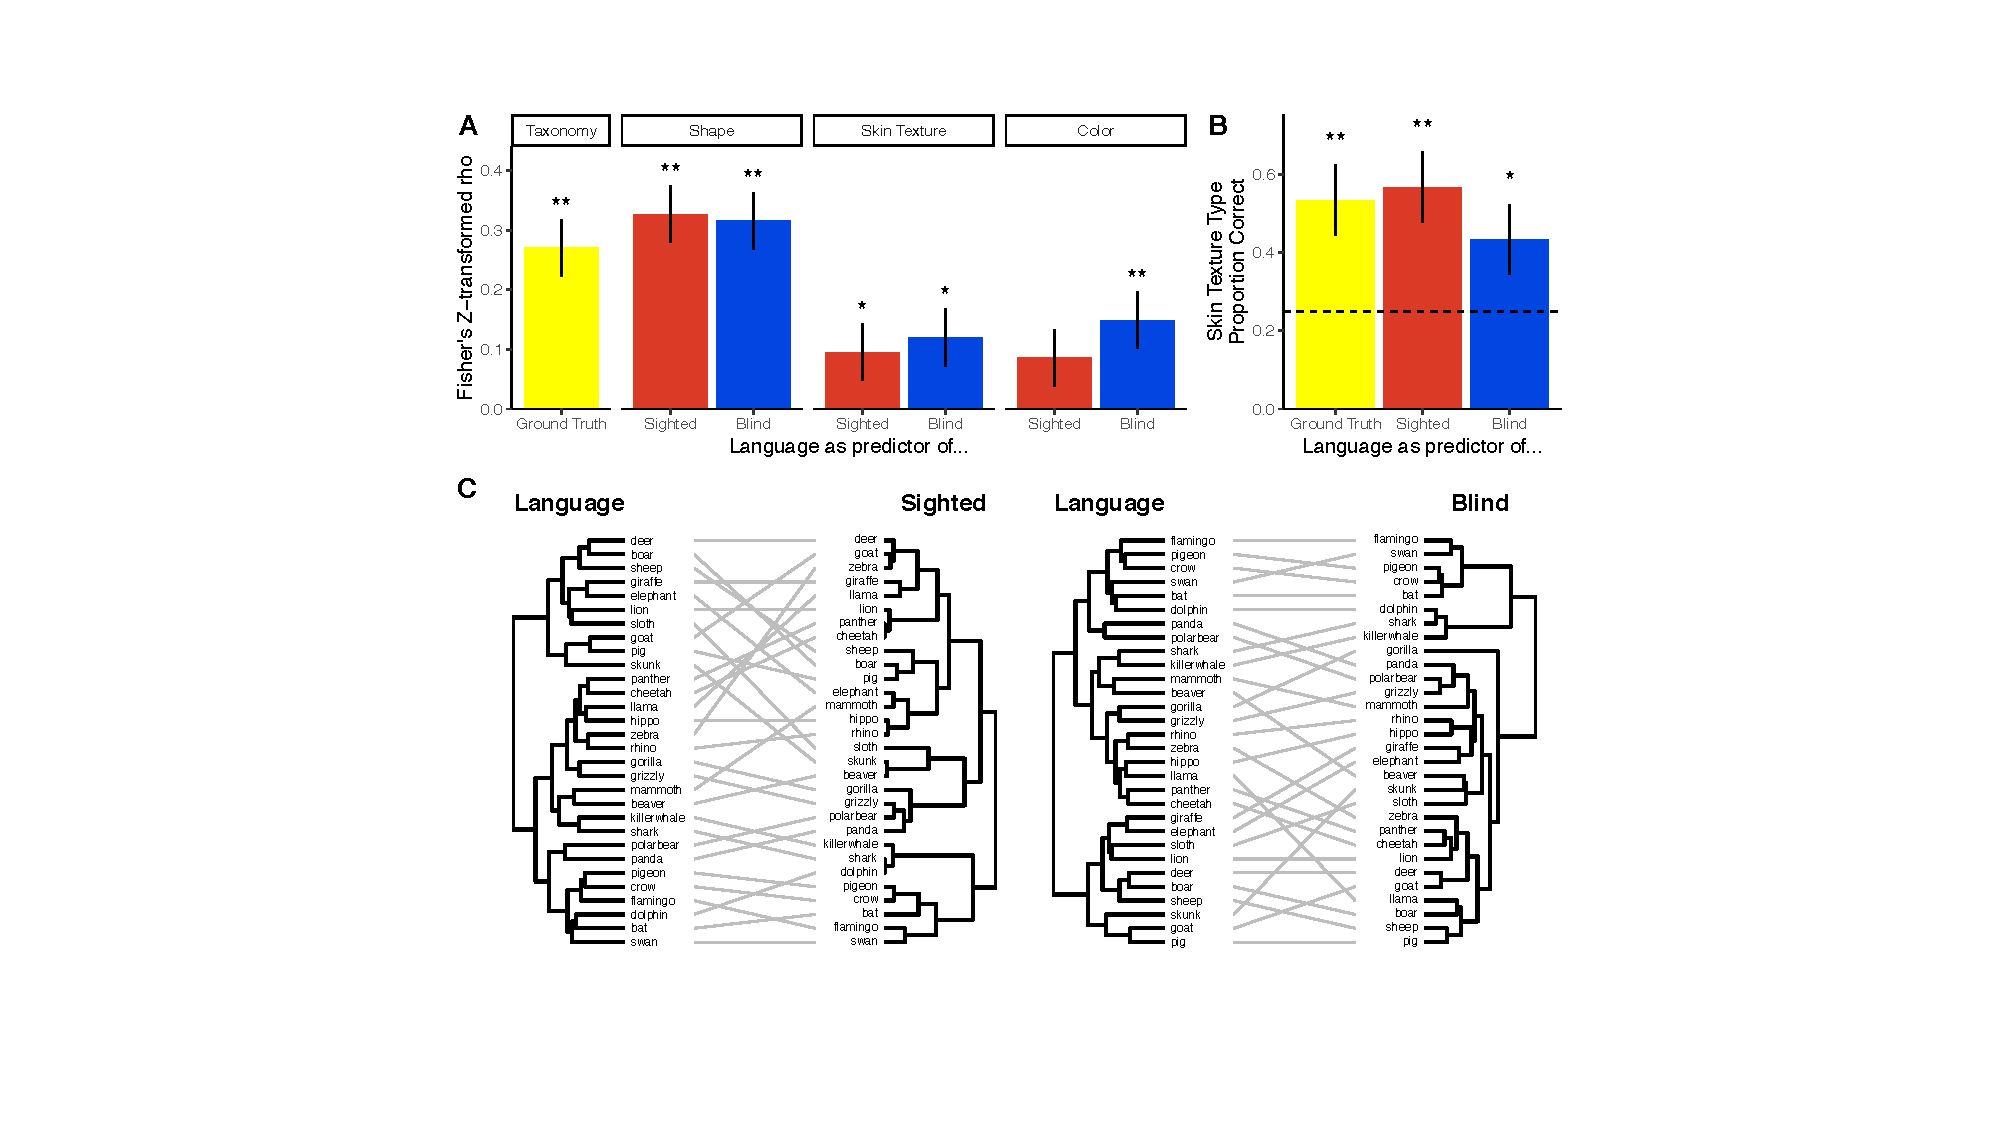
\includegraphics[width=7in]{figureppt3.pdf}
      \caption{\footnotesize  A.\ Pairwise correlations (Fisher transformed as in 1) between language-derived animal similarities (cosine distances) and evolutionary distances (yellow), performance of sighted (red) and blind (blue) participants. Human comparisons are shown separately for shape, skin texture, and color card-sorting tasks in (1). B.\ Language statistics classify animals as having scales, skin, fur, or feathers at levels well-above chance. Predictive accuracy is shown for ground truth (yellow) and performance of sighted (red) and blind (blue) participants.  C.\ Relationships among animals computed entirely from language statistics show considerable overlap with relationships derived from shape-based categorization produced by sighted (left) and blind (right) participants. The labels in the two language-based dendrograms are ordered to maximize alignment with behavioral data. Single asterisks indicate \textit{p} $<$  .05; Double asterisks indicate \textit{p} $<$ .01. }
\end{figure}

\subsubsection*{References}

1. 	Kim JS, Elli GV, Bedny M (2019) Knowledge of animal appearance among sighted and blind adults. {\it Proc Natl Acad Sci} 116(23):11213–11222.
\vspace{3mm}

\noindent2. 	Mikolov T, Chen K, Corrado G, Dean J (2013) Efficient estimation of word representations in vector space. {\it ArXiv Prepr ArXiv13013781}. Available at: \url{https://arxiv.org/abs/1301.3781} [Accessed March 23, 2017].
\vspace{3mm}

\noindent3. 	Bojanowski P, Grave E, Joulin A, Mikolov T (2016) Enriching Word Vectors with Subword Information. {\it ArXiv160704606 Cs}. Available at: \url{http://arxiv.org/abs/1607.04606} [Accessed April 5, 2017].
\vspace{3mm}

\noindent4. 	Hill F, Reichart R, Korhonen A (2016) Simlex-999: Evaluating semantic models with (genuine) similarity estimation.  {\it Comput Linguist.} Available at: \url{http://www.mitpressjournals.org/doi/abs/10.1162/COLI_a_00237} [Accessed April 4, 2017].
\vspace{3mm}

\noindent5. 	Gerz D, Vulić I, Hill F, Reichart R, Korhonen A (2016) Simverb-3500: A large-scale evaluation set of verb similarity.  {\it ArXiv Prepr ArXiv160800869}. Available at: \url{https://arxiv.org/abs/1608.00869} [Accessed April 4, 2017].
\vspace{3mm}

\noindent6. 	Bedny M, Koster-Hale J, Elli G, Yazzolino L, Saxe R (2019) There's more to ``sparkle'' than meets the eye: Knowledge of vision and light verbs among congenitally blind and sighted individuals.  {\it Cognition} 189:105-115.

\end{document}
